\documentclass[11pt]{article}
\usepackage[a4paper,margin=2cm]{geometry}
\usepackage{amsmath}
\usepackage{enumitem}
\usepackage{booktabs}
\usepackage{array}
\usepackage{graphicx}
\usepackage{parskip}
\setlist{itemsep=3pt, topsep=3pt}
\newcommand{\menu}[1]{\textbf{#1}}

\begin{document}

{\LARGE\bfseries CoAP test: laptop $\leftrightarrow$ NodeMCU}\\[4pt]
The laptop asks the NodeMCU for its stats (\texttt{GET /stats}) and can switch the NodeMCU's blue LED on and off (\texttt{PUT /led}). No broker.

\section*{Files in this folder}
\begin{tabular}{@{}>{\ttfamily}l l@{}}
nodemcu\_coap\_server/nodemcu\_coap\_server.ino & CoAP \textbf{server}. Arduino sketch (C++) for the NodeMCU. \\
coap\_client.py & CoAP \textbf{client}. Python script for the laptop. \\
\end{tabular}

\section*{How it fits together}
\begin{center}
\texttt{coap\_client.py (laptop)} $\xrightarrow{\ \mbox{\small GET /stats, PUT /led}\ }$ \texttt{NodeMCU (server)}\\[2pt]
\texttt{coap\_client.py (laptop)} $\xleftarrow{\ \mbox{\small 2.05 Content + data}\ }$ \texttt{NodeMCU (server)}
\end{center}

\begin{tabular}{@{}>{\raggedright}p{3.4cm} >{\raggedright}p{6.2cm} >{\raggedright\arraybackslash}p{6.6cm}@{}}
\toprule
 & \textbf{MQTT} (previous test) & \textbf{CoAP} (this test) \\
\midrule
Broker & Yes (Mosquitto) & \textbf{No}: laptop talks to the board directly \\
Who starts & NodeMCU \textbf{pushes} every 2 s & Laptop \textbf{asks}, NodeMCU \textbf{answers} \\
Transport & TCP, port 1883 & \textbf{UDP}, port \textbf{5683} \\
Feels like & a group chat & a tiny website for devices (GET / PUT, like HTTP) \\
NodeMCU role & client (publisher) & \textbf{server} \\
\bottomrule
\end{tabular}

\vspace{6pt}
The NodeMCU offers three things (``resources''):
\begin{itemize}
\item \texttt{GET /stats} $\rightarrow$ JSON: \texttt{uptime\_s}, \texttt{rssi\_dbm}, \texttt{free\_heap}, \texttt{a0} (same meaning as in the MQTT test).
\item \texttt{GET /led} $\rightarrow$ \texttt{on} or \texttt{off}.
\item \texttt{PUT /led} with payload \texttt{on} / \texttt{off} $\rightarrow$ switches the blue LED.
\end{itemize}
\texttt{2.05 Content} in the answers is CoAP's version of HTTP's ``200 OK''.

\textbf{Network:} the laptop and the NodeMCU must be on the \textbf{same Wi-Fi}. No internet, no broker and \textbf{no proxy} are needed:
the traffic is local. Tested working on the college Wi-Fi (IIITA). A phone hotspot also works.

\newpage
\section*{Step 1: Install the libraries (once)}
\begin{enumerate}
\item Arduino IDE $\rightarrow$ \menu{Tools $\rightarrow$ Manage Libraries\dots} $\rightarrow$ search \textbf{CoAP simple library} $\rightarrow$ install the one by \textbf{Hirotaka Niisato}.
\item Laptop (PowerShell): \texttt{pip install aiocoap}
\end{enumerate}
(On the college network, Arduino IDE needs its proxy set to download the library:
\menu{File $\rightarrow$ Preferences $\rightarrow$ Network $\rightarrow$ Manual proxy}, host \texttt{172.31.2.3}, port \texttt{8080}.)

\section*{Step 2: Open and edit the sketch}
\menu{File $\rightarrow$ Open} $\rightarrow$ \texttt{nodemcu\_coap\_server/nodemcu\_coap\_server.ino}, then set the Wi-Fi at the top:
\begin{verbatim}
const char* WIFI_SSID = "IIITA";   // Wi-Fi name
const char* WIFI_PASS = "";        // Wi-Fi password ("" if none)
\end{verbatim}
Wi-Fi must be \textbf{2.4 GHz}. There is no broker or proxy setting: CoAP talks directly.

\section*{Step 3: Upload and get the NodeMCU's IP}
\begin{enumerate}
\item Select board \textbf{NodeMCU 1.0 (ESP-12E Module)} and the COM port, then \menu{Upload}.
\item \menu{Tools $\rightarrow$ Serial Monitor}, \textbf{9600 baud}, press \textbf{RST}. It prints:
\begin{verbatim}
Wi-Fi OK. CoAP server ready at  coap://172.29.0.146/stats
>>> Use this IP in coap_client.py <<<
\end{verbatim}
\item Note the IP. Tip: select it in the Serial Monitor and \textbf{Ctrl+C} to copy, instead of typing it.
\end{enumerate}

\section*{Step 4: Ask for the stats from the laptop}
\begin{verbatim}
cd C:\path\to\coap_test
python coap_client.py 172.29.0.146
\end{verbatim}
Every 2 seconds:
\begin{verbatim}
13:17:11 2.05 Content  {"uptime_s":25,"rssi_dbm":-79,"free_heap":49624,"a0":4}
\end{verbatim}
At the same time the Serial Monitor shows \texttt{GET /stats from <laptop IP> -> \{...\}}. Stop with \textbf{Ctrl+C}.

\section*{Step 5: Switch the LED from the laptop}
\begin{verbatim}
python coap_client.py 172.29.0.146 led on
python coap_client.py 172.29.0.146 led off
\end{verbatim}
Answer: \texttt{2.05 Content on} / \texttt{off}. The blue LED on the board follows, and the Serial Monitor shows \texttt{PUT /led 'on' from \dots}.

\section*{Troubleshooting}
\begin{tabular}{@{}>{\raggedright}p{5.4cm} >{\raggedright\arraybackslash}p{10.8cm}@{}}
\toprule
\textbf{Symptom} & \textbf{Cause / fix} \\
\midrule
\texttt{no answer (timeout)} & Wrong IP (check Serial Monitor, press RST), board not powered, or the network blocks UDP between devices: use a phone hotspot for both. \\
Stuck on \texttt{Connecting to Wi-Fi.....} & Wrong name/password, 5 GHz network, or a login page network. \\
Gibberish in Serial Monitor & Baud must be 9600. One short line of gibberish right after RST is normal (boot message). \\
IP changed & The Wi-Fi gives out IPs automatically; it can change after a restart. Read it again from the Serial Monitor. \\
\bottomrule
\end{tabular}

\newpage
\section*{Result (tested)}
Left: \texttt{coap\_client.py} polling \texttt{/stats}, then \texttt{led on} and \texttt{led off}.
Right: NodeMCU Serial Monitor showing each request it answered.

\vspace{6pt}
\begin{center}
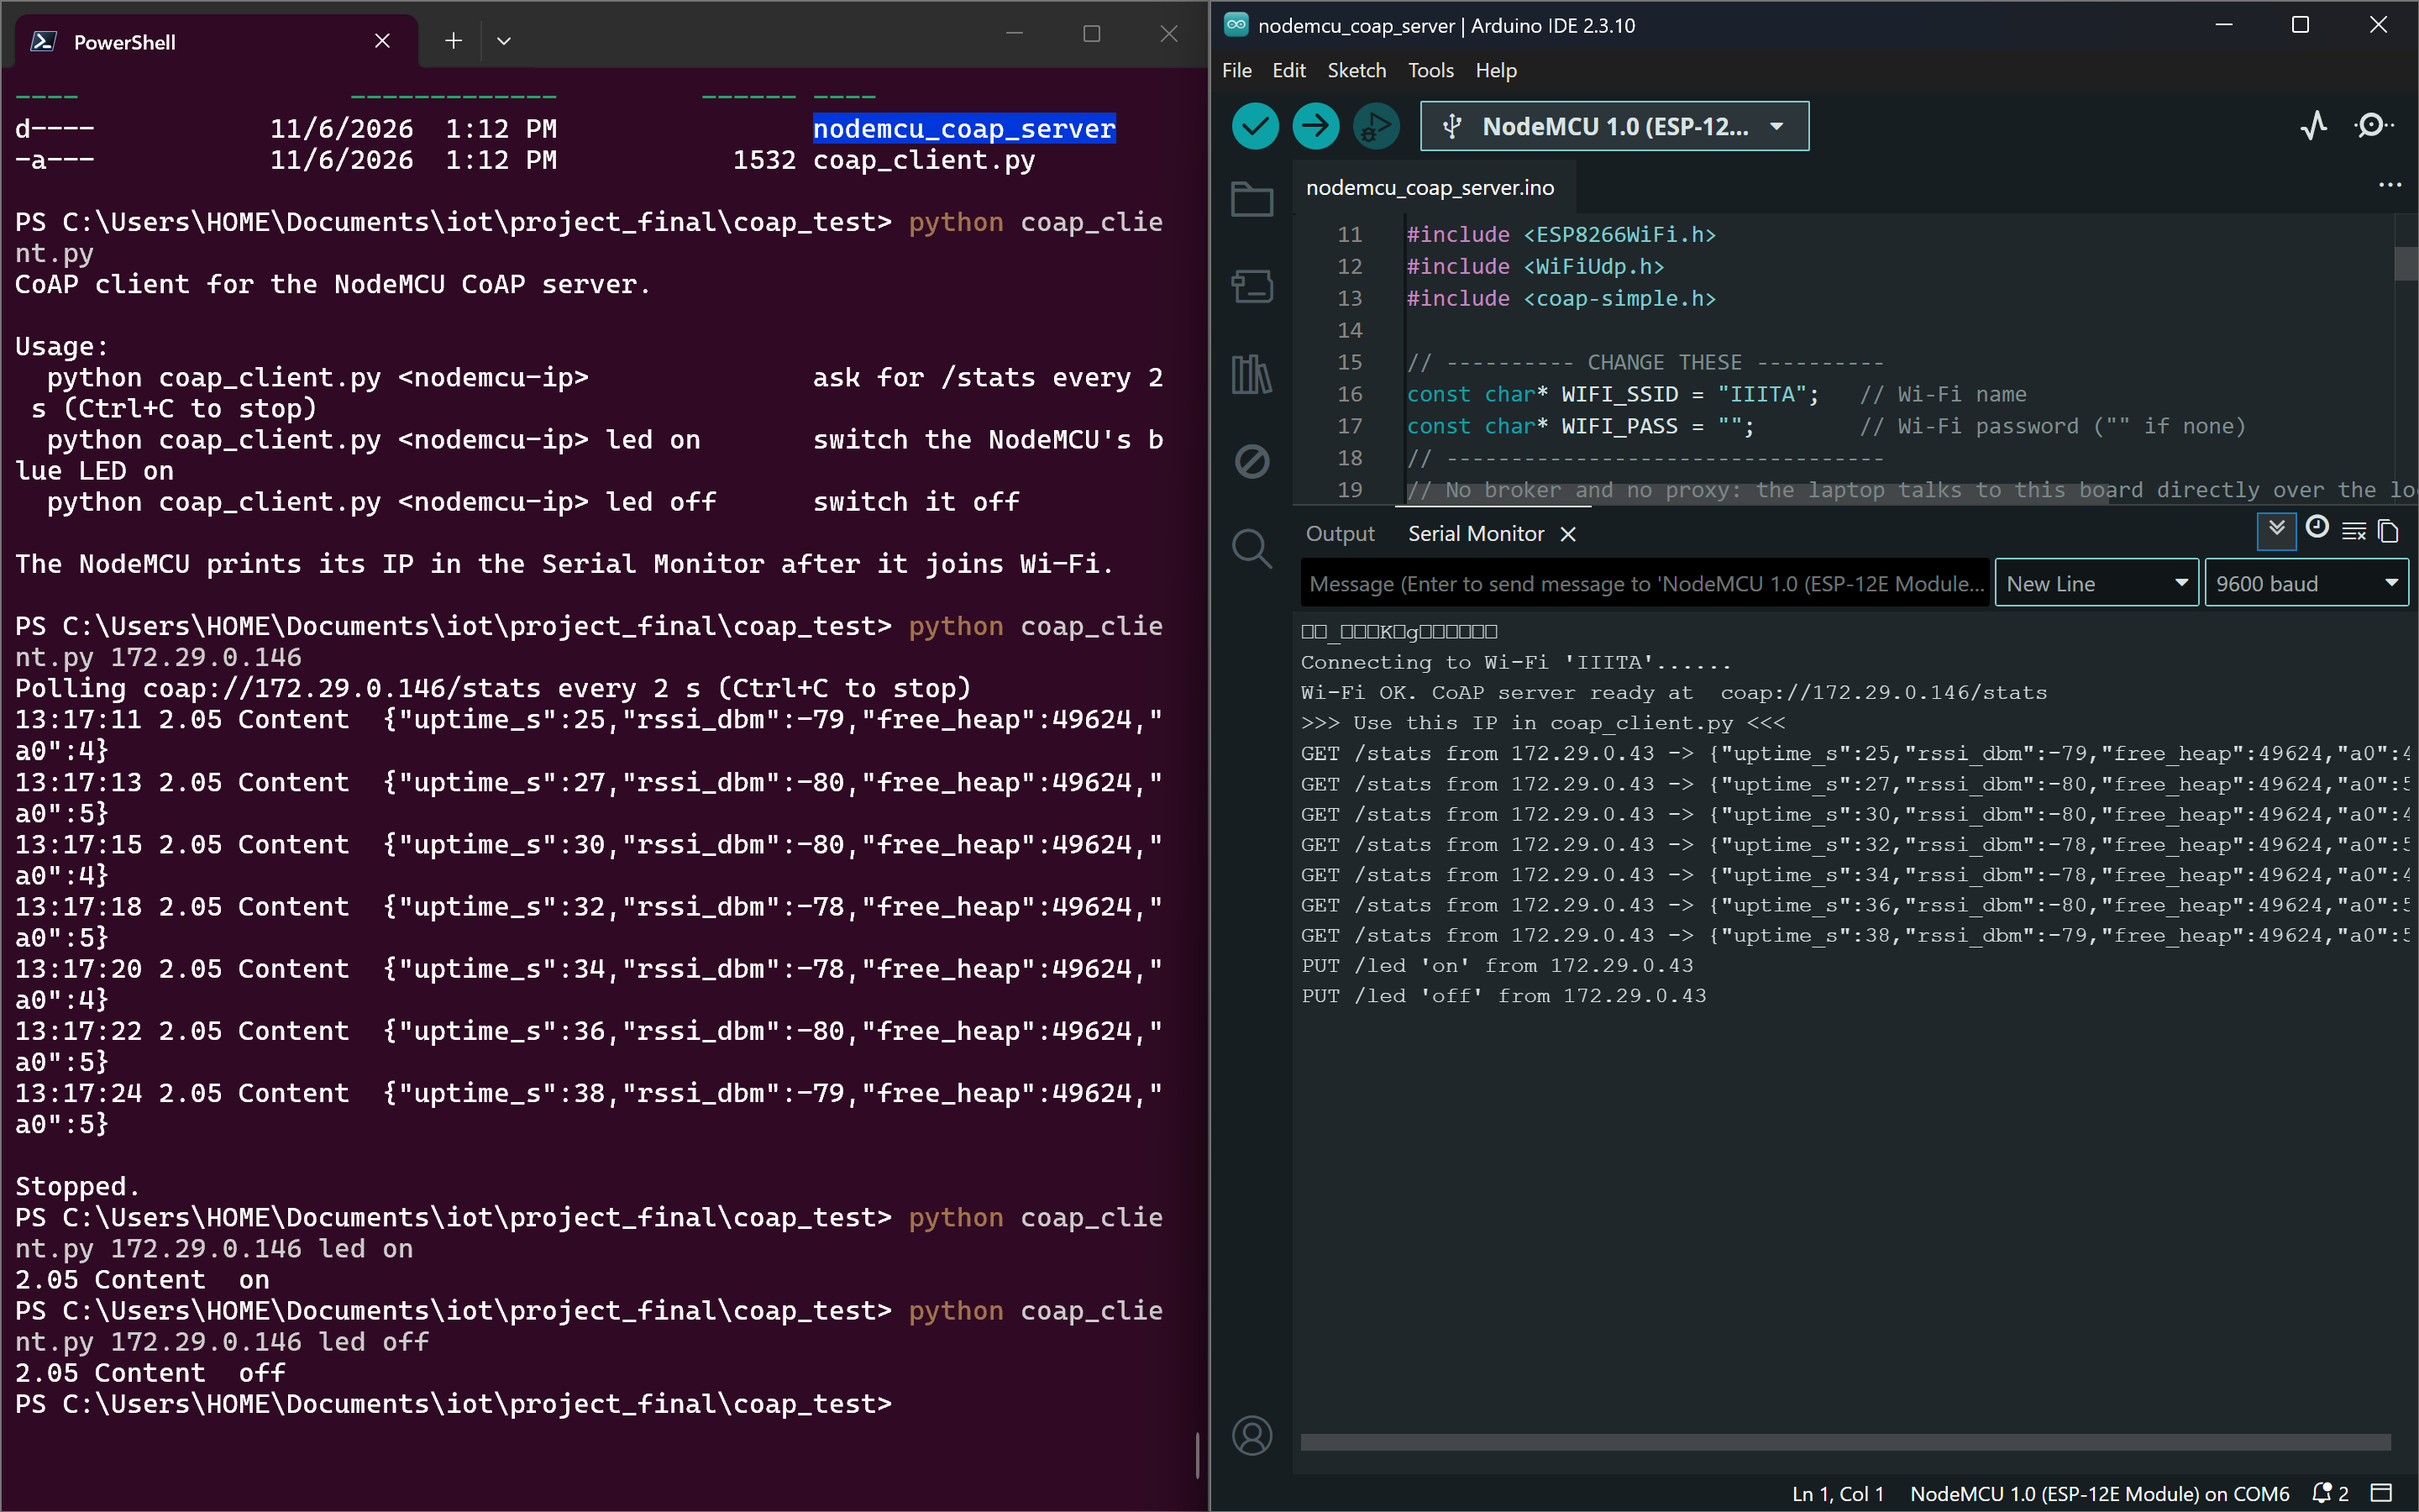
\includegraphics[width=\textwidth]{img/coap_result.png}
\end{center}

\end{document}
